\chapter{Discussion}
\label{chapter:discussion}

This chapter is the analysis of the results and the research process itself. First the research outcomes as answers to the research questions are presented one by one. After summarizing the main findings
and analysis on them, the validity of the research process itself is discussed by considering different threats and how they were addressed during this study. The discussion ends by suggesting
topics for a more detailed research in the future.

\section{Research outcomes}
\label{section:outcomes}

The main outcomes of this study are summarized and analyzed here. The more detailed background information on them is presented in
chapters \ref{chapter:current-state}, \ref{chapter:proposal} and \ref{chapter:evaluation}, respectively.

\subsection{The main problems in the initial state}

The first research question aimed to identify the main challenges in the initial maintenance process. During the initial state analysis, it was evident that the transition from previous the ad hoc process to
the new structured process based on Freshdesk was still ongoing. This became clear during the first workshop, when the official process diagram raised discussion about how the process was actually working, which
was quite far from the official model. One of the most significant problems was considered to be informal communication channels, which were used partly because the customers preferred them, but also partly
because Freshdesk had only five user licenses available at the time, which was clearly not enough for an organization of 16 people. The problem of using informal communication channels was frequent knowledge loss and unclear
initial requirements, because once the email or Slack messages finally reached the person responsible for working on the issue, some parts were quite often missing and the original request could even be
misunderstood because of this. Usage of informal communication channels was also effectively hiding the maintenance tasks from the official process as they rarely resulted in tickets, which makes
organizing maintenance and development tasks challenging and results in multitasking. Additionally it was also considered that Freshdesk had usability issues related to the email client and search functionality
for example, which was also one of the reasons keeping the communication out of the official process.

Judging by the challenges related to informal ad hoc processes, it can be stated that QOCO is a typical small software company. The development of QOCO's maintenance process has been almost identical to
the model proposed by \citet{Hasan2011} (see figure \ref{fig:hasan-flow}). Lacking the sufficient amount of resources to run proper structured processes easily leads to a situation where tasks are handled
on an ad hoc basis by certain key personnel, which leads to further challenges while the company grows. Limited resources is a challenge for small companies \citep{Basri2010}, which can not be entirely solved
without growing the company itself. However, the difficulties caused by it should be addressed with special attention, once there are more resources available.
Also the usability issues on communication tools experienced at QOCO is a well known knowledge sharing barrier described by \citet{Ghobadi2016}, for
example, and therefore it can be stated that the challenges identified in this study are generally in line with the literature.

Another challenge not exactly related to the process itself was knowledge sharing in general. This was mostly visible as a gap on project knowledge between the executives, namely the CTO and COO,
and other employees. There were many reasons for this situation, one of them being the long history of the company as a small startup, which had recently grown rapidly. The processes were not following
the growth of the company, which resulted in many tasks being handled by the CTO and COO without time to share the knowledge to others. This was already noticed at the company, but not much had
been done to solve the issues as their root causes were unclear. According to the knowledge sharing survey during the initial state analysis, the most significant knowledge sharing barriers were considered to be
tight schedule, multitasking and lack of informal documentation (see section \ref{section:survey-results-before}). After a further review it was evident that multitasking was particularly a problem of the executives and the Airline 1 development team.
The overall feeling of time pressure and constantly switching between different tasks effectively reduces, or even entirely prevents, knowledge sharing as it is considered that there is no extra time
to discuss with colleagues about different matters, even though it would be beneficial for the future development.

All of the knowledge sharing barriers identified in this study were already described in previous research by \citet{Ghobadi2016}, \citet{Dalkir2013} and \citet{Riege2005}
for example (see section \ref{section:barriers}), and in that sense this study
supports the findings of the existing literature. Especially lack of documentation in agile methodologies is a well known issue \citep{Ito2016}\citep{Sommerville2011}\citep{Stettina2013}
and as it was a significant issue at QOCO as well, this study further confirms the findings of the previous studies.
Lack of documentation is also closely related to an inadequate transition model between development
and maintenance phases pointed out by \citet{Ito2016} and \citet{Stettina2013} for example. As such model is not defined at QOCO, this study further confirms this relationship. Therefore it can be generally stated
that the challenges found in this study are well in line with the existing literature.

Another point to note is the implications of multitasking on inadequate portfolio management \citep{Vahaniitty2010}. As this was not the main topic to be studied in the scope of this
study, no definite conclusions can be drawn one way or another. However, as QOCO has a growing number of projects with maintenance responsibility, portfolio management
is a topic that should be further addressed in the near future.

After discussing about the findings and their criticality with the executives, there was a mutual understanding that the knowledge sharing issues were the most important ones to be addressed. This was due to
their effect on daily activities, but they also posed a significant threat to company's scaling plans in the future and therefore they had to be solved one way or another. Improvements on the maintenance process
itself were considered also important, but still secondary compared to the knowledge sharing challenges, although knowledge sharing also improves processes and vice versa. In addition to solving the
initial problems, it was also important to not introduce new ones to the process. Therefore it was considered as a loose requirement to not worsen external metrics, such as average resolution times.

\subsection{The most suitable solutions to identified problems}

The second research question focused on finding solutions to the problems identified by the first question. This was done by analyzing existing literature
to gather solutions that could be applicable to the case company's context. The literature review together with
the initial ideas from the first workshop yielded 11 suggestions in total that were then evaluated with the executives to filter out the ones that were not suitable to the case company's overall business strategy.
Seven solution proposals made it through the initial business critical filtering and these proposals were presented to a wider audience of employees in the second workshop to evaluate their suitability and
select the most promising ones to be implemented. As a result, four solution proposals were selected to the implementation phase, although it was suggested that pair working is combined together with rotating
triage responsibility. Other two solutions were README template and project presentations.

The main solution to address the issues in both knowledge sharing and the process itself was considered to be rotating triage responsibility combined with pair working.
To reduce the workload of the CTO and COO on
resolving maintenance tasks, the role of a triage responsible was introduced. The renewed process model with the triage responsible is presented in figure \ref{fig:ticketing-renewed}. The idea of the triage role
is to check all newly reported tickets before they are assigned to a person responsible for resolving them. As QOCO is still a small company, the automatic process suggested by \citet{Hu2014} is not sufficient
in its context and therefore the solution was to handle the triaging process manually although it will not scale very well in the future.
The main task of the triage responsible was to ensure that Freshdesk tickets were reported with enough details and that tags, priorities and
categories were used correctly. After this the ticket would be ready to be assigned for a person responsible for solving it.
The person responsible for triage was rotated on a daily basis, which was considered a useful practice. First of all, this ensures that
there is always someone assigned for triaging on each day, but also it is a transparent and fair way to distribute the triage workload equally to all participants. This way the challenge of decreasing motivation
described by \citet{Faegri2009} could be minimized, but of course not entirely eliminated. As said, the initial five licenses was
far from enough to properly operate the renewed support model and therefore the number of licenses was increased to ten, which was already enough to cover most of the developers and consultants. This should
be enough for now, but if the company continues to grow with a similar rate, it will not be long before the amount needs to be reconsidered again, depending on the organizational structure and other factors of
course.

\begin{figure}[H]
	\begin{center}
		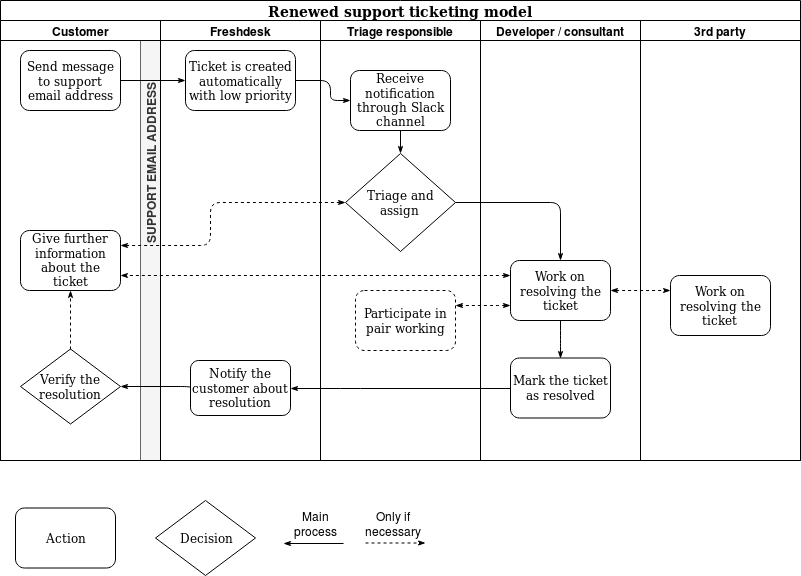
\includegraphics[width=.9\textwidth]{images/Renewed_support_process.png}
		\caption{Renewed process for handling low, medium and high priority incidents}
		\label{fig:ticketing-renewed}
	\end{center}
\end{figure}

Pair working was also added as a part of the triage process to further improve knowledge sharing. The main goal of combining pair working with the triage responsibility was to
share knowledge between the executives and other employees and therefore
reduce dependability on key persons, which was considered a significant threat for scalability. The intended implementation of pair working was that small and well-defined maintenance tasks could be solved by
working as a pair so that the person normally responsible for handling the ticket acts as a navigator and the other person acts as a driver and actually does the tasks at hand, while being instructed by
the navigator. To lower the barrier of finding a pair, it was agreed that the person with the triage responsibility on that day
should be the first candidate to be considered, but of course in some cases it is more suitable and
meaningful to pair with someone else and therefore this was not strictly enforced. Additionally a pair working guide introducing the methodology was created to clarify the practicalities, since all of the
participants were not fully familiar with the principles beforehand.

An additional solution to improve knowledge sharing and prevent knowledge loss over time was to improve the quality of informal documentation. Initially the documentation available was usually either heavy delivery
documentation, delivered to the customer together with a new release, or a few most likely outdated sentences on a README file alongside the codebase. A general README file template was created to tackle
this issue and lower the barrier of writing at least a few more sentences about the intended use case and development instructions while developing the project itself. The template was considered a useful solution
since as discussed in the second workshop, writing a README file is easily forgotten and considered too troublesome, when there are no general guidelines about its contents easily available. The template was
considered easy to implement with a potential of significant improvements and therefore it was selected for the implementation phase. The template was stored on the company's GitHub account for easy accessibility
and version control.

Another solution to tackle the dependability on key persons and lower the barriers between different teams was to have project presentations on a regular basis. The main goal of the presentations was to
share general knowledge about business cases without going deeply into technical details. The presentations were intended to be kept short and informal to ensure that they would not become a mandatory burden
for anyone. To ensure informality, relaxed atmosphere and a wide audience, it was agreed that these presentations would be added as an occasional part of the weekly Friday meetings that were highly casual and usually without any
predetermined agenda. Therefore a short 10 minute presentation would not take much time from casual chatting and could act as a "topic of the day" -like inspiration, although it was not necessarily meant to
be like that.
	
\subsection{Effectiveness of the selected solutions}

The purpose of the third research question was to analyze how well the implemented solutions managed to address the challenges identified by RQ1. This effectiveness was measured by
using various metrics presented in section \ref{section:measuring}.
These metrics formed a base for the goals of the implementation phase, which were prioritized into three categories: primary, secondary and optional. Next
each of the goals with different priority levels are evaluated based on the results of the implementation phase presented in section \ref{section:metric-results}.

\subsubsection*{Primary goals}

The primary goals that were the main focus area of this study were aiming to address the challenge of knowledge sharing, which was considered as one of the main challenges of the organization.
The challenge was especially sharing knowledge between the executives and other employees since due to company's background, the CTO and COO handled most of the maintenance tasks in the initial maintenance process.
The overall goal was to share the maintenance responsibility and skills so that the workload would be more equally distributed and the executives would have more time available for new development and
management tasks.

The first goal of decreasing the gap between the executives and others at 3+ level (G1) directly addressed the problem of maintenance tasks piling up on the CTO and COO. The gap was initially 6.3 projects for juniors and
8.8 for seniors, but during the implementation phase, the executives actually increased their knowledge at 3+ level, while others remained unchanged (see table \ref{table:projects-per-level-after}). Therefore this goal was not fulfilled as the gap actually increased
rather than being decreased. The reason for this is that the executives, namely the CTO and COO, had quite many projects initially on level 2, which were then increased to level 3 during this study.
The common denominator for the projects with increased knowledge levels was that they were all older legacy projects that are not familiar for many employees in the company. The use of outdated technologies
also introduced further challenges with knowledge sharing on legacy projects, since they were developed years ago by the CTO and employees who are no longer working at the company. Therefore the current employees are not
familiar with the used technologies, which limits the possibility of knowledge sharing. This is an issue emphasized by \citet{Richardson2007}, which could become increasingly problematic in the future, however
it is not a significant challenge at QOCO yet, although it is still a thing to be aware of.

Despite the increased gap on 3+ level, it is also notable that the executives actually lost knowledge on level 5, while juniors managed to increase their knowledge (see table \ref{table:projects-per-level-after}).
This is highly positive as the gap on level 5
knowledge was also large between the executives and others and these changes confirm that the solutions have actually managed to share the responsibility and the most detailed knowledge about newer projects.
By analyzing the responses in a more detailed manner, it is evident that this change is indeed caused by newer projects still in active development mode. As the projects are being developed further, the
complexity usually increases and keeping knowledge up to date requires continuous effort. Therefore the fact that the gap between the executives and juniors has decreased on level 5 knowledge is a sign
of successful knowledge sharing between the executives and juniors. However, it is unclear whether this was caused by the implemented solutions or not, but at least they have most likely had
a positive impact on this development.

The second primary goal of increasing persons per project on 3+ level (G2) reflected the diversity of the skill sets. As the time frame of this study was limited, it was agreed that the focus should be on
increasing persons with 3+ knowledge, because it represents all employees with enough knowledge to do at least minor tasks on the project. Initially the amount was 3.2 for an average project and the goal was
to increase it to 4.0 during the implementation, which was quite ambitious. The amount was actually increased to 3.6 (see figure \ref{fig:skill-distribution-after}), which is only half of the intended improvement, but still a significant positive
change. Therefore this goal was only partially fulfilled, but the direction of the development is definitely right and should continue in the future as well. It is still notable that this increase is mainly
explained by the increase on the executives' knowledge, which was not exactly the intended outcome of this study and therefore the future development should focus more on increasing the knowledge of other employees as
well.

The third and fourth primary goals were related to lowering the significance of knowledge sharing barriers. First of all, tight schedule and multitasking (G3) are quite closely related to each other, and they were
initially considered as the main barriers for sharing maintenance knowledge. The most significant effect was on tight schedule as its significance score decreased by 5
(see section \ref{section:knowledge-metrics-after}), although it was still considered
as the most significant barrier. The effect on multitasking was not that strong, but it also managed to decrease its score, which fulfills G3. However, multitasking still remains a challenge as all teams have
actually increased their multitasking factor during the study (see table \ref{table:toggl-after}), even though the overall feeling was that the triage process has decreased the interruptions and multitasking.
The situation is especially worrying on the Airline 1 development team, which has a significantly high multitasking factor compared to other teams. This is a challenging
managerial issue, which should be addressed soon to prevent it from getting even worse.

As described previously, multitasking could be a sign of inadequate portfolio management \citep{Vahaniitty2010}, but its root cause in QOCO's context was not extensively studied in the scope of this study.
Tight scheduling on the other hand is a typical issue of small companies with limited resources \citep{Kajko-Mattsson2009}, which is in line with the fact that it remains the most significant knowledge sharing
barrier also at QOCO even after this study. Since this is the case, further improvements on the situation require a more detailed analysis on the root causes of both multitasking and scheduling issues
as they are closely related to each other.

What comes to lack of informal documentation as a knowledge sharing barrier (G4), it was initially considered as the third most significant barrier, which was then addressed directly by implementing a README
template. The goal itself was fulfilled as the significance of the barrier was lowered, but an even more interesting development was an increased demand for formal documentation, which was a bit surprising.
One explanation for this could be that actually the practice of triaging has raised a demand for documentation, which has been missing in many cases. Additionally there was a concern
about managing multiple parallel documentations, which was discussed during the third workshop.
Informal documentation with the README template could be seen as the first step towards more structured documentation practices
as the documentation has mostly been nonexistent previously. Therefore the development on informal documentation is definitely good as it encourages discussion on documentation practices in a wider context as well.

Lack of documentation is a well known challenge of agile methodologies and it is usually solved by relying on informal documentation and tacit knowledge \citep{Basri2011}\citep{Ersoy2015}\citep{Stettina2013}.
However as it increases the risk of knowledge loss, which has been evident at QOCO as well, it is a positive development that this study has managed to raise discussion about documentation practices in general.
Based on this study, it would be beneficial to include some light documentation to the development process, which is emphasized by \citet{Stettina2013} for example, as it would ease the transition between
development and maintenance phases. However as noted in the third workshop as well, writing documentation to no one in particular is not especially motivating and decreases the documentation quality, which is
also noted by \citet{Stettina2013}. This an important challenge to be carefully considered while developing better documentation practices for QOCO in the near future.

\subsubsection*{Secondary goals}

The three secondary goals were related to the process itself by addressing internally reported tickets, resolution times and the ratio of alerts. They represent the effectiveness of the solutions from process
improvement point of view, which was not considered as critical as the primary challenges related to knowledge sharing, but still highly valuable. The changes in underlying metrics for these goals have been
presented in section \ref{section:process-results}.

First of all, there was a goal to increase the ratio of alerts from initial 7 \% to 10 \% (G5) since it would reflect better customer service and an improved quality of incoming tickets. Distribution of ticket types after
the implementation phase is presented in figure \ref{fig:ticket-types-after} and based on that graph, it is evident that this goal was not fulfilled. The ratio of alerts between January and April was only 2 \%,
which marks a significant drop from the initial ratio of 7 \%. Also the absolute number of alerts decreased by 67 \% compared to a 4-month average of 2018 and therefore the decrease in ratio can not be explained
by an increased total amount of tickets. One explanatory factor that mostly explains the decrease is the fact that most alerts in 2018 were caused by network connectivity issues on a single application. This has been
apparently fixed as there has not been any more alerts related to that between January and April.

Secondly, it was intended that the ratio of internally reported tickets would decrease from initial 10 \% to 5 \% (G6) since it would mean that more tickets are reported directly to the support email address by
customers rather than being forwarded by QOCO's employees. However there was also a challenge on this goal as an increasing ratio of internally reported tickets would also mean that an increasing amount of
previously hidden tasks have been reported to the official process and it seems like that this is exactly what happened. The goal itself was not fulfilled as the ratio of internally reported tickets increased
to 19 \%, meaning that it almost doubled from the initial value (see figure \ref{fig:ticket-domains-after}). However, also the ticket count increased significantly during the implementation phase
(see figure \ref{fig:resolution-times-after}) and therefore it
most likely means that an increasing amount of tickets are being actually reported to the support email address rather than being solved outside of the Freshdesk process. This is a good thing for now, but since the
ratio is as high as 19 \% currently, it is a clear point of improvement in the future since approximately one out of five newly created tickets are not initially reported to the support email address by the customers.

The last process improvement goal was to solidify the average resolution time below 30 hours during the implementation phase (G7). As can be seen from the figure \ref{fig:resolution-times-after}, the average resolution time
for low priority tickets varied between 12 and 51 hours between January and April, and between 12 and 37 hours during the implementation in March and April. Therefore it can be argued that the goal is not
exactly fulfilled, but it is still worth noting that the average resolution time during the implementation phase
in March and April was 24 hours, which is below the goal. Also an average resolution time of 12 hours in April marks a record
low of the observation period while the ticket count has significantly increased and therefore the solutions have proved their worth even though the goal was not exactly fulfilled. This development was thought
to be mainly due to improved assignment practices with the triage responsibility. As initially new tickets were waiting for "someone" to take action on them, the triage process ensures that the newly reported
tickets are directly assigned to the person responsible for solving them, which decreases the overall resolution time as can be observed from the data. It is notable that the time period is still too
short to claim that the average resolution time has been solidified and therefore it needs to be confirmed in the future when there is more data available.

\subsubsection*{Optional goals}

In addition to the primary and secondary goals, there were also two optional goals that were considered as nice additions, but not necessary the ones to be focusing on. First of all, it was considered positive if
the ratio of low priority tickets was decreased from initial 94 \% to 90 \% (G8), since it was thought that the priorities were not used correctly in Freshdesk and some higher priority tickets could be
misclassified as low priority as it was the default for new tickets. However this goal was not fulfilled since the ratio of low priority tickets remained unchanged at 94 \% after the implementation phase.
Therefore it is arguable that there are most likely not that much misclassifications as the process has been better structured and there has been more concern towards the correct usage of priority levels.
It can also be explained by a coincidence since the time period is only four months and higher priority tickets are still quite rare, which could mean that the ratio could increase with a longer time period,
but there is no data to confirm that in the scope of this thesis. Either way, as this goal was considered optional, it is not that critical to continue monitoring in the future.

The second optional goal was to keep the total amount of tickets between 40 and 50 monthly tickets (G9). This would mean that the implemented solutions do not introduce more incidents that require
maintenance actions, although an increase in ticket amount could also be explained by more tickets being actually reported to the official process. This goal has definitely not been fulfilled as the average
amount of tickets in March and April was approximately 70 (see figure \ref{fig:resolution-times-after}), which exceeds the goal by a great margin.
As already argued above, this is mostly due to an increasing amount of previously hidden tickets being
reported to the support email address, which causes the total amount to increase even though the actual workload remains the same. This hypothesis is also confirmed by an increased ratio of internally
reported tickets and a more detailed look into the source data, which confirmed that the tickets were not directly caused by the implemented solutions. It is also worth noting that keeping the ticket amount below
a certain limit does not necessarily reflect the effectiveness of the development or maintenance processes, since an increasing amount of different projects and a growing business should generally result in
an increase in support tasks as well. With this in mind, the exact amount of tickets is not something to worry about, although it is still good to check the underlying reason if rapid growth is experienced
in the future.

\subsubsection*{Implications and conclusions}

To conclude the answer to the third research question, the goals and their outcomes are gathered to the table \ref{table:goal-results} for easier evaluation. Judging by the goals it can be stated
that this study has been successful, although it is clear that there is still a lot of work to be done in the future. As three of the primary goals were either fulfilled or partially fulfilled, it can be
argued that the implemented solutions seem to have successfully addressed the identified challenges and they have managed to improve the internal processes.
This naturally does not imply that these solutions are universally suitable for all small software companies, but it definitely encourages further studies on the subject.

\begin{table}
	\begin{center}
		\begin{tabular}{|c|c|c|}
			\hline
			\textbf{Goal} 	& \textbf{Priority} & \textbf{Result}                                                                                                 			\\ \hline
			G1 & Primary 	& \begin{tabular}[c]{@{}c@{}}Not fulfilled. The gap actually increased on 3+ level\end{tabular}              									\\ \hline
			G2 & Primary 	& \begin{tabular}[c]{@{}c@{}}Partially fulfilled. The amount of persons \\ at 3+ level increased from 3.2 to 3.6\end{tabular}						\\ \hline
			G3 & Primary 	& \begin{tabular}[c]{@{}c@{}}Fulfilled. The significance of tight schedule \\ decreased by 5 points and multitasking by 1 point\end{tabular}       	\\ \hline
			G4 & Primary 	& \begin{tabular}[c]{@{}c@{}}Fulfilled. The significance decreased by 1 point\end{tabular}                       									\\ \hline
			G5 & Secondary 	& \begin{tabular}[c]{@{}c@{}}Not fulfilled. The ratio decreased from 7 \% to 2 \%\end{tabular}                                              			\\ \hline
			G6 & Secondary	& \begin{tabular}[c]{@{}c@{}}Not fulfilled. The ratio increased from 10 \% to 19 \%\end{tabular}                                 						\\ \hline
			G7 & Secondary 	& \begin{tabular}[c]{@{}c@{}}Partially fulfilled. \\ The average of March and April was 24 hours\end{tabular}                               		\\ \hline
			G8 & Optional 	& \begin{tabular}[c]{@{}c@{}}Not fulfilled. \\ The ratio of low priority tickets was unchanged\end{tabular}                               			\\ \hline
			G9 & Optional 	& \begin{tabular}[c]{@{}c@{}}Not fulfilled. The average of March and April \\ was roughly 70 tickets per month \end{tabular}                		\\ \hline
		\end{tabular}
		
		\caption{Summary of the results}
		\label{table:goal-results}
	\end{center}
\end{table}

Based on this study, I would argue that the rotating triage responsibility is a viable option to be considered in small software companies that are struggling to transform ad hoc maintenance processes
into more structured ones. The clear benefits of it are that it will encourage knowledge sharing and communication between teams, but also generally improve the efficiency of the maintenance process by shared
responsibility. As all of the issues addressed in this study were quite typical for a small software company growing rapidly \citep{Hasan2011}, the rotating triage responsibility should be applicable to
other similar companies as well. Also since most of the literature on triaging practices focuses on automatic triaging in large companies (\citet{Hu2014} for example),
it would be scientifically interesting to implement
a similar solution in another context to get further insight on its applicability on a more general level.

Based on these findings, combining triage responsibility with pair programming or pair working is not exactly necessary from the process point of view,
although it encourages knowledge sharing and communication. This study confirms that implementing
pair programming in an actual case is quite difficult. The main challenges on pair working were considered to be its resource intensity
and task selection. These findings are in line with the previous research on the subject, such as \citet{Lui2010}, \citet{Plonka2012} and \citet{Spohrer2013},
and therefore the suitability of pair working for small and highly specialized companies is questionable.

The implications on the informal documentation highlight the contradiction on README files, since they should be written when they are needed the least. As discussed, the documentation should be added
as a part of the handover practices, even if using agile methodologies \citep{Stettina2013}, which should be mutually agreed by the team. A problem of motivation and creating good quality
content still remains, although the template has improved
the quality significantly. The documentation practices of the case company will require further iterations in the near future, but it seems like the template has started the discussion, which is a good first step
of the continuous improvement.

On the process improvement point of view QOCO is also a typical small company with a high commitment on process improvement, but lacking the resources and methodology to implement it \citep{Basri2010a}. 
As a key takeaway from this study, the company has implemented one iteration using continuous improvement methodology and as a result, has a better understanding of its present challenges and possible methods to
address them. This study managed to raise discussion about internal process improvement and existing challenges, which marks an important change in the mindset of the whole organization. The success of the
process improvement in the context of this study encourages the use of similar methods in other cases as well.

\section{Threats to validity}

To be able to understand the trustworthiness of this study, it is important to understand the precautions taken in the research design and during the research process. Validity of this study directly evaluates
the trustworthiness of the presented results and therefore before making any further implications, it should be addressed from different perspectives. \citet[p.~71-72]{Runeson2012} divide
validity into four categories:
\emph{construct validity, internal validity, external validity} and \emph{reliability}. Each of these aspects and precautions taken to improve them are discussed below.

\subsection{Construct validity}

Construct validity refers to interpretation issues in measures under research, including interview questions and selected metrics for example \citep{Runeson2012}. This study utilized several data collection
methods and therefore there are many opportunities for interpretation issues. First of all, the executives were interviewed several times during the study, but the interviews were unstructured rather than
being structured and standardized as a qualitative study method. During the interviews it was ensured that both the researcher and the executives understood the topics in the same way by asking more detailed questions
and ensuring that both parties had a similar understanding on the subject. It is also notable that the researcher had a long background in the company and there was already a trust relationship and common understanding of 
the topics before the study, which reduces the risk of misunderstandings.
Even though the interviews were not audio recorder, the discussed topics were on a general level and rather than relying on single quotes from these
discussions, the study relied on overall understanding. Therefore it can be argued that the risk of interpretation issues on interviews is low.

Similarly, workshops as a main data collection method for qualitative data is subject to interpretation issues. For example discussed topics could have been understood differently by different employees, but
this was addressed by creating an open environment of discussion, which encourages to ask for clarifications if something is unclear. These clarifications and confirmations on discussed topics were quite
common during the workshops and judging by the outcomes, it can be stated that the risk of interpretation issues was also well handled.

In addition to the workshops and interviews there was also a survey for quantitative data analysis about knowledge sharing. The risk of interpretation issues on survey is much higher than in previous methods since
it was answered individually, although there was a possibility to ask for clarifications if questions were unclear. However, this does not entirely remove the risk of misunderstandings and different
interpretations and it is possible that the respondents understood for example the difference between skill levels differently.
To lower this risk, the survey was used to measure the initial state and the outcome after the
study. By keeping the survey exactly the same between the measurements and analyzing the overall change rather than each individual response separately, the risk of misinterpretations does not have
that large impact on validity of the results. It is still worth noting that the population of the survey was very small, which increases the impact of individual misinterpretations.

One additional data collection method used was analyzing data exports from ticket and time tracking systems. As the data export analysis relies on selected metrics, it is important to consider how well these metrics actually represent
the studied topic. This was addressed by evaluating 12 software maintenance metrics from literature and 10 custom defined metrics tailored for the case company's context. The metrics were analyzed together with
the executives, which resulted in selecting seven most suitable ones to be used. Because of this careful evaluation, it can be argued that the selected metrics most likely represent the studied topic quite well and therefore
the overall construct validity is high.

\subsection{Internal validity}

Internal validity refers to explaining causality and analyzing the factors outside this study that could have affected the results \citep{Runeson2012}. What comes to this study and its results, it can not
be explicitly stated that the results occurred purely because of the actions taken in the scope of this study. Because there was no control group that could be used as a reference point, the results could
be entirely caused by external factors and not this particular study. To tackle this issue this study utilized multiple data sources for triangulation and did not rely on a single data source on the implications.
Also the results and their interpretations were discussed together with the executives to find possible alternative explanations for them.
This reduces the risk of external factors affecting the results, but does not entirely remove it. Therefore it can be concluded that there is no solid proof of high internal validity, but the necessary precautions
have been taken to ensure that it would be as high as possible.

\subsection{External validity}

External validity analyzes the applicability of the results on a more general context \citep{Runeson2012}. It is clear that this study is extremely
context dependent and a similar study in another context could yield entirely different results. Also the time period was quite short meaning that the results should not be used to draw any long term general
implications, although they could be used as a reference point for other studies on the subject. More generalizable results to define a general theory
would require additional studies in similar contexts. To improve repeatability of this
study, the research process has been documented in detail including used methods, the context and practicalities. Therefore the study itself should be repeatable, but the results might be entirely different. 
It can be argued that the external validity of this study is low due to high dependency on its context, but the possible actions to improve repeatability have been taken.

\subsection{Reliability}

Reliability of a study refers to its dependence on the researcher \citep{Runeson2012}. As the researcher had worked at the case company for over a year already before starting the study, the objectivity is
questionable. However, the history at the case company could also be seen as a positive aspect since driving organizational change is much easier as an already agreed member of the community,
rather than being newly introduced. This most likely affects the results of this study, because organizational change is a complex outcome of social interactions after all and another researcher outside
the case company, or even inside of it, could have entirely different results. Despite of this, repeatability of the study has been improved by documenting all the data collection and analysis methods
in detail, although using unstructured interviews is not optimal in this sense. The implications of the data analysis during different phases of the study were also discussed with the executives to find
alternative explanations, which reduces the risk of biased analysis of the researcher, although does not remove it entirely.
The interview and workshop topics have been documented, together with the used Think-Pair-Share methodology, but there
could still be open questions about the details of them, which reduces repeatability. Also the study itself is no longer entirely repeatable in the same organization because
it has already been conducted once and resetting the context back to the initial setting is no longer possible. Therefore it can be concluded that reliability of this study is questionable, but the research
design and methodology have been documented to allow repeating a similar study in a different context.

\section{Future research}

As discussed already in the previous section, this study is highly context dependent and should not be used as the only source of general implications. To get a more general understanding of software maintenance
challenges in small organizations and ways to solve them,
a similar study could be repeated in multiple different organizations. Then this study could act as a single data point in a larger multiple case study, which then could yield
more generalizable results about the challenges and the applicability of the solutions of this study. As a wider scope for future studies, a suggestion based on this study is to
further research maintenance processes in general and their relationship to development workflow, especially in the context of small organizations. This could also yield more suggestions about the best practices
on how to effectively manage an increasing amount of maintenance tasks together with active development.

Another important aspect that did not fit to the scope of this study was handover practices in agile organizations, both small and large. The agile methodology usually handles mostly the management of development
tasks, but does not have much attention on maintenance tasks. It is almost like the software is forgotten after it has been released, which is far from reality. As agile methodologies do not generally emphasize 
extensive documentation, handover from active development to maintenance is risky and potentially results in knowledge loss. This is even the case when there is no separate maintenance team and the project
is handed over to the development team itself by shifting it to maintenance mode. Therefore it is suggested that agile handover practices should be studied more as it is an important phase in 
software development in general, but it has not been studied extensively in the agile context.

Also the suitability of pair working for small companies raised questions that were left unanswered in this study. Judging by the results it seems that pair working is inherently unsuitable for small companies
as the need for resources is in contradiction with the fact that lack of resources is one of the key problems of small organizations. The case is especially difficult in highly specialized companies where also
the task selection and pairing become problematic. The benefits are also more applicable for larger companies as they focus
on improved knowledge sharing and code quality. Therefore a further confirmatory study could be arranged to test this hypothesis on different sized companies.

Another important aspect especially for the case company, but also in a more general context, is to have further studies on how to detect software faults before they become an issue. The natural answer to this
is by improving monitoring, but the tricky part is detecting the right events while not reporting an extensive amount of false positives. This was identified as an interesting and important topic during the 
initial interviews of this study, but it was not advanced any further due to vague definitions of responsibilities and the limited time period. Therefore it remains to be solved in the case company, but it would
also be interesting to research further in other cases as well.

What comes to the specific context of the case company, I would suggest that the suitability of different agile methodologies in a highly regulated field of aviation industry could be further evaluated. Also the
recent development towards implementing different standards to gain competitive advantage could be another topic for further research since highly standardized processes are not in line with the agile ideology
and the literature argues that small organizations do not generally like to implement standards. Therefore their implementation needs to be carefully planned and there could be another research assignment on a topic
related to this. In addition to entirely new topics, it is also worth noting that this study was only the first iteration of continuous process improvement that could be further implemented in the future, since
without continuous improvement, the outcome of this study will most likely also face issues after a while.
